\chapter{Experiments}

% feedback Benjamin
% Structuur sectie
% Eerst in kleine sectie experimenten oplijsten
% Subsecties
% - Experiment 1
% - Experiment 2
% Experimenten is ruimte om resultaten te schrijven
% Eerste observaties

% Explain first which experiments are done and why
% Per section: - Write down results of experiments

\section{Localization evaluation}
We evaluate the five \acrshort{wsol} methods that are described in detail in section \ref{lb:wsol_methods}: CAM, GradCAM, GradCAM++, ScoreCAM and MinMaxCAM. All these methods, except GradCAM, are evaluated using a VGG-GAP network and a Resnet-50 network. GradCAM is a generatization of CAM that yields the same score maps as CAM in a \acrshort{cnn} with \acrshort{gap} layer like the VGG16-GAP and ResNet-50 networks. GradCAM, GradCAM++ and ScoreCAM are also evaluated using a VGG16 network. As these methods don't require an architecture with \acrshort{gap} layer, it is interesting to see how they perform on the unmodified VGG16 architecture.

We evaluate the models on a synthetic dataset and on the ImageNet dataset. For the VGG16-GAP network and the ResNet-50 network, we trained two models per network on the synthetic dataset: One without regularization and one with MinMaxCAM regularization. For the VGG16 network we only train one model on the synthetic dataset as MinMaxCAM is not compatible with this network. Evaluation on the ImageNet dataset is done on pre-trained networks, except for MinMaxCAM which requires training due to its regularization stage.

\subsection{Synthetic dataset}
We evaluate the \acrshort{cam} methods on the synthetic datasets listed in Table \ref{tab:synthetic_datasets}, using the MaxBoxAccV3 and PxAP metrics. In following sections, results for VGG16-GAP, VGG16 and ResNet-50 architectures are discussed.

\subsubsection{VGG16-GAP}
The localization results using the multiple-instance \acrshort{wsol} metric MaxBoxAccV3 are shown in Table \ref{tab:maxboxaccv3_vgg16_gap_synthetic}. The pixel average precision results are illustrated in Table \ref{tab:pxap_vgg16_gap_synthetic}. From the results, some interesting observations can be noticed.
\begin{table}[ht]
\centering
\begin{tabular}{lrrrrrrrr}
\toprule
 & \multicolumn{8}{c}{VGG16-GAP synthetic (MaxBoxAccV3)} \\
method & d1b & d1t & d2b & d2t & d3b & d3t & d4b & d4t \\
\cmidrule(lr){1-1} \cmidrule(lr){2-9} 
cam & 93.67 & 91.67 & 66.58 & 65.67 & 60.94 & 59.11 & 48.67 & 54.87 \\
gradcam++ & 94.17 & \bfseries 92.50 & 67.33 & 65.08 & 62.50 & 59.11 & 48.42 & 55.17 \\
minmaxcam & \bfseries 94.83 & 89.33 & 67.33 & 65.17 & 62.83 & 57.67 & 48.87 & 43.33 \\
scorecam & 94.17 & 88.83 & \bfseries 73.00 & \bfseries 68.08 & \bfseries 69.33 & \bfseries 65.11 & \bfseries 51.37 & \bfseries 56.58 \\
\bottomrule
\end{tabular}
\caption[MaxBoxAccV3 for VGG16-GAP on synthetic datasets]{MaxBoxAccV3 for VGG16-GAP on synthetic datasets.}
\label{tab:maxboxaccv3_vgg16_gap_synthetic}
\end{table}
\begin{table}[h]
\centering
\begin{tabular}{lrrrrrrrr}
\toprule
 & \multicolumn{8}{c}{VGG16-GAP synthetic (PxAP)} \\
method & d1b & d1t & d2b & d2t & d3b & d3t & d4b & d4t \\
\cmidrule(lr){1-1} \cmidrule(lr){2-9} 
cam & 80.82 & 80.45 & 78.52 & 74.68 & 76.31 & 72.79 & 65.69 & 72.55 \\
gradcam++ & \bfseries 81.82 & \bfseries 81.56 & \bfseries 79.33 & \bfseries 74.96 & \bfseries 77.90 & 73.20 & 66.92 & 73.21 \\
minmaxcam & 81.29 & 80.46 & 78.62 & 74.00 & 75.44 & 71.43 & 66.10 & 57.24 \\
scorecam & 80.71 & 81.07 & 77.96 & 74.32 & 77.64 & \bfseries 75.10 & \bfseries 67.34 & \bfseries 73.45 \\
\bottomrule
\end{tabular}
\caption[PxAP for VGG16-GAP on synthetic datasets]{PxAP for VGG16-GAP on synthetic datasets.}
\label{tab:pxap_vgg16_gap_synthetic}
\end{table}

\textbf{Multi-instance localization performance} drops with increasing object instances. MaxBoxAccV3 is above or close to 90\% for the single instance datasets d1b and d2b. A significant performance difference exists for 2-instance and 3-instance datasets, compared with single instance datasets. Localization performance is worst for the dataset with four instances per image, although still about half of all object instances can be localized with a model that is trained for classification only.

\textbf{Pixel average precision} doesn't drop as significantly as MaxBoxAccV3 for images with multiple object instances. Intuitively, a reasonable explanation is a mismatch at pixel-level causes a less severe penalty than a mismatch at the coarse-grained bounding box level.

\textbf{Best MaxBoxAccV3 for multiple instances} is obtained by ScoreCAM. The promising results for multi-target visualization observed by Wang \textit{et al.} \cite{wang2020score}, seem to hold in our quantitative evaluation.

\subsubsection{VGG16}
The localization results for VGG16 on the synthetic datasets are shown in Table \ref{tab:maxboxaccv3_vgg16_base_synthetic} for the MaxBoxAccV3 metric and in Table \ref{tab:pxap_vgg16_base_synthetic} for the PxAP metric. Note that CAM and MinMaxCAM methods cannot be used on VGG16 as this architecture has no \acrshort{gap} layer. GradCAM is used here as generalization of CAM.

\begin{table}[ht]
\centering
\begin{tabular}{lrrrrrrrr}
\toprule
 & \multicolumn{8}{c}{VGG16 synthetic (MaxBoxAccV3)} \\
method & d1b & d1t & d2b & d2t & d3b & d3t & d4b & d4t \\
\cmidrule(lr){1-1} \cmidrule(lr){2-9} 
gradcam & \bfseries 82.83 & \bfseries 77.33 & \bfseries 56.08 & 37.33 & \bfseries 55.17 & 44.39 & 48.79 & 40.21 \\
gradcam++ & 77.00 & 70.83 & 40.92 & 26.83 & 47.39 & 37.33 & 40.17 & 34.08 \\
scorecam & 81.83 & 74.50 & 55.00 & \bfseries 44.58 & 54.44 & \bfseries 48.56 & \bfseries 51.04 & \bfseries 45.79 \\
\bottomrule
\end{tabular}
\caption[MaxBoxAccV3 for VGG16 on synthetic datasets]{MaxBoxAccV3 for VGG16 on synthetic datasets.}
\label{tab:maxboxaccv3_vgg16_base_synthetic}
\end{table}
\begin{table}[h]
\centering
\begin{tabular}{lrrrrrrrr}
\toprule
 & \multicolumn{8}{c}{VGG16 synthetic (PxAP)} \\
method & d1b & d1t & d2b & d2t & d3b & d3t & d4b & d4t \\
\cmidrule(lr){1-1} \cmidrule(lr){2-9} 
gradcam & \bfseries 71.14 & \bfseries 65.89 & 60.66 & 42.86 & 61.69 & 46.63 & 56.26 & 50.54 \\
gradcam++ & 66.88 & 59.54 & 49.45 & 29.74 & 56.42 & 40.43 & 50.40 & 39.47 \\
scorecam & 69.19 & 65.12 & \bfseries 61.79 & \bfseries 50.66 & \bfseries 62.64 & \bfseries 56.56 & \bfseries 58.82 & \bfseries 56.15 \\
\bottomrule
\end{tabular}
\caption[PxAP for VGG16 on synthetic datasets]{PxAP for VGG16 on synthetic datasets.}
\label{tab:pxap_vgg16_base_synthetic}
\end{table}

We see the same trends as noticed for the VGG16-GAP network. An additional observation is that the localization metrics for VGG16 are lower than those of the VGG16-GAP network on the same datasets. Intuitively, in the VGG16 network there is a less direct relationship between feature activation in the last convolutional layer and the predicted target due to the dense network between the convolutional backbone and the classification output.

\subsubsection{ResNet-50}
Localization performance results for the ResNet-50 network on the synthetic dataset are illustrated in Table \ref{tab:maxboxaccv3_resnet50_synthetic} for MaxBoxAccV3 and in Table \ref{tab:pxap_resnet50_synthetic} for PxAP. Here GradCAM is not evaluated as it performs the same as CAM for architectures with a \acrshort{gap} architecture.

\begin{table}[ht]
\centering
\begin{tabular}{lrrrrrrrr}
\toprule
 & \multicolumn{8}{c}{ResNet-50 synthetic (MaxBoxAccV3)} \\
method & d1b & d1t & d2b & d2t & d3b & d3t & d4b & d4t \\
\cmidrule(lr){1-1} \cmidrule(lr){2-9} 
cam & 82.83 & 65.50 & 62.00 & 60.67 & 63.44 & 59.61 & 57.67 & 52.62 \\
gradcam++ & \bfseries 83.83 & 67.67 & \bfseries 63.67 & 65.08 & 65.39 & 61.67 & \bfseries 60.79 & 53.58 \\
minmaxcam & 75.33 & 60.67 & 57.58 & 48.92 & 52.00 & 53.72 & 54.33 & 49.92 \\
scorecam & 80.50 & \bfseries 69.67 & 62.33 & \bfseries 66.25 & \bfseries 65.44 & \bfseries 63.44 & 58.83 & \bfseries 56.17 \\
\bottomrule
\end{tabular}
\caption[MaxBoxAccV3 for ResNet-50 on synthetic datasets]{MaxBoxAccV3 for ResNet-50 on synthetic datasets.}
\label{tab:maxboxaccv3_resnet50_synthetic}
\end{table}

\begin{table}[ht]
\centering
\begin{tabular}{lrrrrrrrr}
\toprule
 & \multicolumn{8}{c}{ResNet-50 synthetic (PxAP)} \\
method & d1b & d1t & d2b & d2t & d3b & d3t & d4b & d4t \\
\cmidrule(lr){1-1} \cmidrule(lr){2-9} 
cam & 71.89 & 57.79 & 70.16 & 71.97 & 71.62 & 70.04 & 69.90 & 64.32 \\
gradcam++ & \bfseries 73.03 & 60.93 & \bfseries 71.48 & 73.88 & \bfseries 72.50 & 70.79 & \bfseries 70.55 & 64.91 \\
minmaxcam & 60.47 & 48.43 & 63.95 & 55.16 & 61.16 & 61.90 & 65.72 & 59.95 \\
scorecam & 72.27 & \bfseries 61.78 & 69.77 & \bfseries 74.18 & 71.30 & \bfseries 72.62 & 68.78 & \bfseries 65.77 \\
\bottomrule
\end{tabular}
\caption[PxAP for ResNet-50 on synthetic datasets]{PxAP for ResNet-50 on synthetic datasets.}
\label{tab:pxap_resnet50_synthetic}
\end{table}

A similar trend as for VGG16-GAP and VGG16 networks can be observed: Localization performance decreases for increasing number of object instances in images. ScoreCAM has the highest MaxBoxAccV3 score for most datasets, while GradCAM++ scores best on the ones where ScoreCAM has lower scores. When looking at the PxAP scores, GradCAM++ scores highest at the datasets with background, and ScoreCAM outperforms the other methods for the datasets without background.

Chattopadhay \textit{et al.} \cite{chattopadhyay2017grad} illustrate visually how taking a weighted combination of positive partial derivatives instead of a global average solves the problem of identifying multiple occurrences of the same class in an image and improper object localization. We quantitatively show that this statement holds when comparing with the other methods.

MinMaxCAM is performing significantly lower than the other methods. Wang \textit{et al.} \cite{wang2021minmaxcam} put in place two conditions for common region regularization to work: Images from the same class should have different background, and features should have different activation values for images with different background. This explains the lower scores for datasets without background (with the one exception for d3b and d3t).

Intuitively, this explains the lower performance for the datasets without background. There is room for improvement by using a hyper parameter search for each dataset and network combination.

\subsection{ImageNet dataset}
In this section we evaluate the \acrshort{cam} methods on the ImageNet validation dataset. Multi-instance localization metric MaxBoxAccV3 is used as in previous sections. In addition we show the MaxBoxAcc and MaxBoxAccV2 metrics to benchmark our trained models with results provided by Choe \textit{et al.} \cite{choe2020evaluating} where appropriate. \acrfull{pxap} cannot be used as the ImageNet dataset has no ground truth segmentation masks. In following sections, results for VGG16-GAP and ResNet-50 architectures are discussed.

\subsubsection{VGG16-GAP}
We modified a pretrained VGG16 network into the VGG16-GAP network by replacing the dense network with a \acrshort{gap} layer and softmax layer. This network is further trained until the loss of the validation dataset hasn't decreased for five consecutive epochs. The localization results of VGG16-GAP on the ImageNet validation dataset are illustrated in Table \ref{tab:metrics_vgg16_gap_imagenet}.

\begin{table}[ht]
\centering
\begin{tabular}{lrrr}
\toprule
method & MaxBoxAcc & MaxBoxAccV2 & MaxBoxAccV3 \\
\cmidrule(lr){1-1} \cmidrule(lr){2-4}
cam & 61.19 & 60.22 & 38.44 \\
gradcam++ & \bfseries 61.29 & \bfseries 60.43 & \bfseries 38.66 \\
scorecam & 58.44 & 57.56 & 36.48 \\
\bottomrule
\end{tabular}
\caption[Metrics for VGG16-GAP on ImageNet]{Metrics for VGG16-GAP on ImageNet.}
\label{tab:metrics_vgg16_gap_imagenet}
\end{table}

The scores for the metrics MaxBoxAcc ($61.19$) and MaxBoxAccV2 ($60.22$) for the \acrshort{cam} method closely match the results documented by Choe \textit{et al.} \cite{choe2020evaluating}. Our VGG16-GAP model is thus able to reproduce the results in the \acrshort{wsol} evaluation paper. MaxBoxAccV3 for ScoreCAM is 2 percentage points lower than CAM and GradCAM++. An intuitive explanation for lower ScoreCAM score could be that ScoreCAM tends to generate more focuses score maps than GradCAM++, resulting in less accurate bounding box estimations. Due to time constraints, MinMaxCAM wasn't trained for the VGG16-GAP network on ImageNet.

\subsubsection{ResNet-50}

For the ResNet-50 network we evaluate four \acrshort{cam} methods on the ImageNet validation dataset. The results are shown in Table \ref{tab:metrics_resnet50_imagenet}. For the \acrshort{cam} method the MaxBoxAcc and MaxBoxAccV2 metrics have lower scores than those reported by Choe \textit{et al.} (57.60 and 57.25 versus 64.2 and 63.7). We used a pre-trained ResNet-50 model where the authors of the mentioned paper did a grid search on hyper parameters to improve localization. The MaxBoxAccV3 metrics has slightly lower values than those for the VGG16-GAP network, but the same trend can be observed. GradCAM++ is the best performing method and ScoreCAM score is 2 percentage point below the GradCAM++ one. MinMaxCAM performs slightly worse than CAM. Wang \textit{et al.} \cite{wang2021minmaxcam} illustrated that MinMaxCAM improves MaxBoxAcc by 2.5 percentage points compared to CAM. We haven't reproduced the results of the authors, due to lack of reference values for the regularization weights. Given the values to reproduce the author's results, the multi-instance localization metric MaxBoxAccV3 could further improve for MinMaxCAM.

\begin{table}[ht]
\centering
\begin{tabular}{lrrr}
\toprule
method & MaxBoxAcc & MaxBoxAccV2 & MaxBoxAccV3 \\
\cmidrule(lr){1-1} \cmidrule(lr){2-4}
cam & 57.60 & 57.25 & 36.58 \\
gradcam++ & \bfseries 59.40 & \bfseries 58.55 & \bfseries 37.53 \\
minmaxcam & 58.81 & 57.26 & 36.02 \\
scorecam & 56.19 & 56.35 & 35.92 \\
\bottomrule
\end{tabular}
\caption[Metrics for ResNet-50 on ImageNet]{Metrics for ResNet-50 on ImageNet.}
\label{tab:metrics_resnet50_imagenet}
\end{table}

%- MaxBoxAcc, PxAP for (vgg16, resnet50), (synthetic, imagenet), CAM methods
%- discuss and explain differences
%- show multiple examples of each method, architecture, dataset
%- discuss and compare results

\section{Threshold calibration}
Different \acrshort{cam} methods exhibit different localization performance distributions, as illustrated in Fig. \ref{fig:boxacc_resnet50_imagenet}. Fixing the operating threshold $\tau$ at a pre-defined value, will increase performance for others. 

Under our threshold-independent performance measures MaxBoxAccV3, we observe that the methods have different optimal threshold $\tau$ (at maximum box accuracy) on ImageNet and the methods do not exhibit significantly different MaxBoxAccV3 performances.

\begin{figure}[ht]
    \begin{center}       
    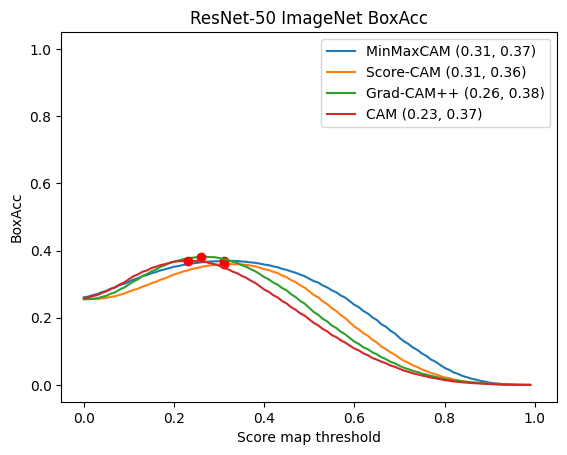
\includegraphics[width=0.7\textwidth]{fig_boxacc_resnet50_imagenet.png}
    \caption[ResNet-50 BoxAcc on ImageNet]{Performance at varying operating thresholds. ResNet-50 on ImageNet: BoxAcc($\tau$) versus score map threshold $\tau$.}
    \caption*{Source: Author}
    \label{fig:boxacc_resnet50_imagenet}
    \end{center}
\end{figure}

\section{Classification versus localization accuracy}
In many cases, the best localization performances are achieved at early epochs, before the classifiers are sufficiently trained. We illustrate this in Fig. \ref{fig:classification_versus_localization} for the MinMaxCAM where we show the training curves of the classification accuracy and localization accuracy on the synthetic validation dataset for the ResNet-50 network. 

\begin{figure}[ht]
    \begin{center}       
    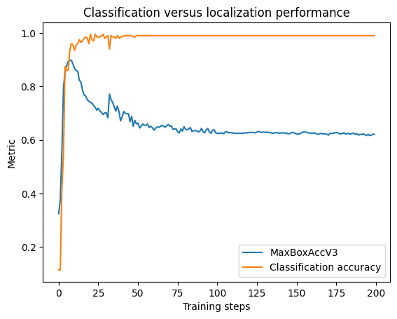
\includegraphics[width=0.7\textwidth]{fig_class_vs_localization.png}
    \caption[Classification versus localization accuracy]{Classification versus localization accuracy comparison of MinMaxCAM method for the VGG16-GAP model on the synthetic dataset.}
    \caption*{Source: Author}
    \label{fig:classification_versus_localization}
    \end{center}
\end{figure}

During the early train epochs, both classification accuracy and localization accuracy improve. When classification accuracy starts to converge, localization performance drops until they both converge.

The result shows that localization and classification performances may not necessarily correlate and further classification training may hurt localization performance. As classification accuracy improves, the model focuses on learning the most discriminative parts of an object to classify the image correctly. These discriminative parts only partially cover an object. As the localization objective is to cover the full object region, improving classification performance decreases localization accuracy. 

Therefore, it's important to use localization-only metrics like MaxBoxAccV3 and PxAP for model selection and evaluation of WSOL methods. To avoid learning a model which focuses on optimizing classification performance only, we stop the learning process when the validation loss hasn't decreased for five consecutive epochs.

\section{Computational complexity}
In this section we evaluation the computational complexity of \acrshort{cam} methods used in our experiments. We measure the runtime of the method as explained in section \ref{sec:computational_complexity}. The method runtime for the ResNet-50 network on the ImageNet validation dataset is illustrated in Table \ref{tab:runtime_resnet50_imagenet}.

\begin{table}[ht]
\centering
\begin{tabular}{lr}
\toprule
method & runtime (seconds) \\
\cmidrule(lr){1-1} \cmidrule(lr){2-2}
cam & 254 \\
gradcam++ & 867\\
minmaxcam & 282 \\
scorecam & \bfseries 106437 \\
\bottomrule
\end{tabular}
\caption[Method runtime for ResNet-50 on ImageNet validation dataset]{Method runtime for ResNet-50 on ImageNet validation dataset.}
\label{tab:runtime_resnet50_imagenet}
\end{table}

The runtime is measured as the total number of seconds it takes to compute score maps for the 50000 images in the ImageNet validation dataset. Runtime exludes operations to load and preprocess the images. GradCAM was not measured as this method specializes to the CAM method for VGG-GAP and ResNet-50. However, it has the same order of complexity as GradCAM++ due to the equal number of forward and backward passes. GradCAM++ takes rougly three times the runtime of the CAM method. This could indicate that backward passes are twice as costly as forward passes.

Each method computes a score map as a weighted combination of feature maps in the final convolutional layer. CAM (MinMaxCAM uses the CAM method for computing score maps), takes as weights the parameters learned in the single fully connected layer, which is a very cheap operation. GradCAM and GradCAM++ compute weights from the backprogagated gradients in the final convolutional layer. Similarly this operation is not computationally expensive.

The most computationally costly method by far is ScoreCAM. This method computes the weights for the feature maps by feeding the network with the product of each feature map with the original image to obtain the classification score after softmax. As ResNet-50 has 2048 channels in its final convolutional layer, this is an expensive operation.

\section{Localization improvements}
